
\newsection
\subsection{BP ?:    %% fill in the BP number
 ??}                 %% fill in the name

\subsubsection{Problem specification}

\begin{itemize}

\item PMEL-135, pp ??

\item Problem description provided by Champion 
      \cite{bp?description}.  %% fill in the problem number

\item Original paper or other sources??

\end{itemize} 


\subsubsection{What we did}

%% Itemize the assumptions we made, etc.

\begin{itemize}
\item  
\end{itemize} 



\subsubsection{Gauge comparisons}


%% SAMPLE FIGURE: %%% Organize your figures in the folder bp? for your problem.

\begin{figure}[ht]

% Two figures side by side:
\hfil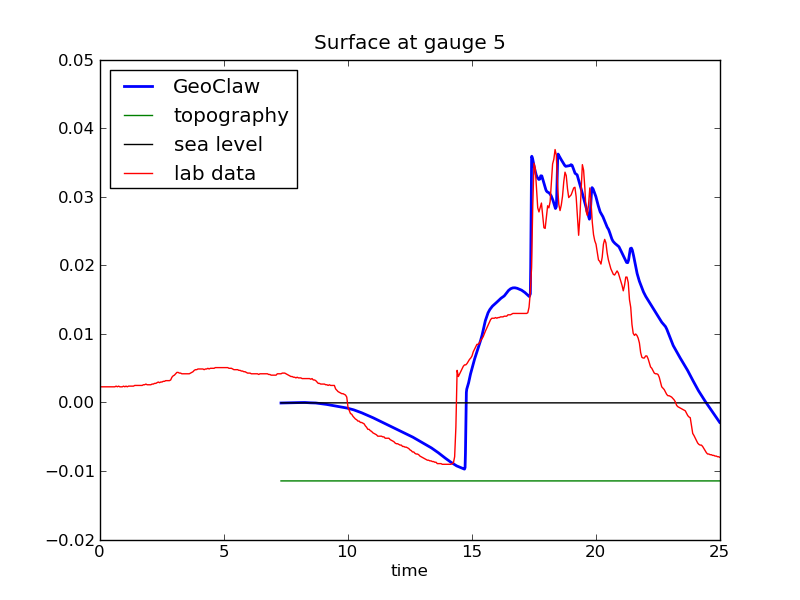
\includegraphics[width=2.8in]{bp7/figs423/gauge0005fig300.png}\hfil
\hfil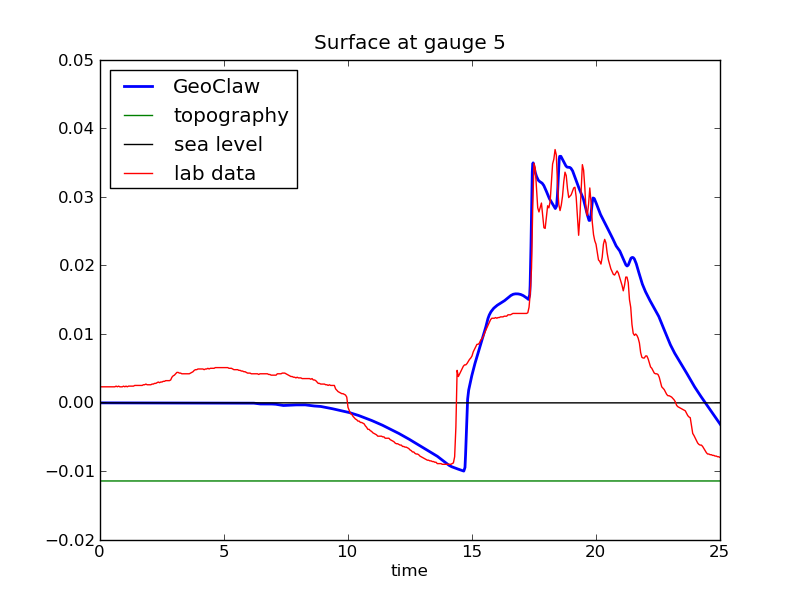
\includegraphics[width=2.8in]{bp7/figs211/gauge0005fig300.png}\hfil

% One wider figure:
\hfil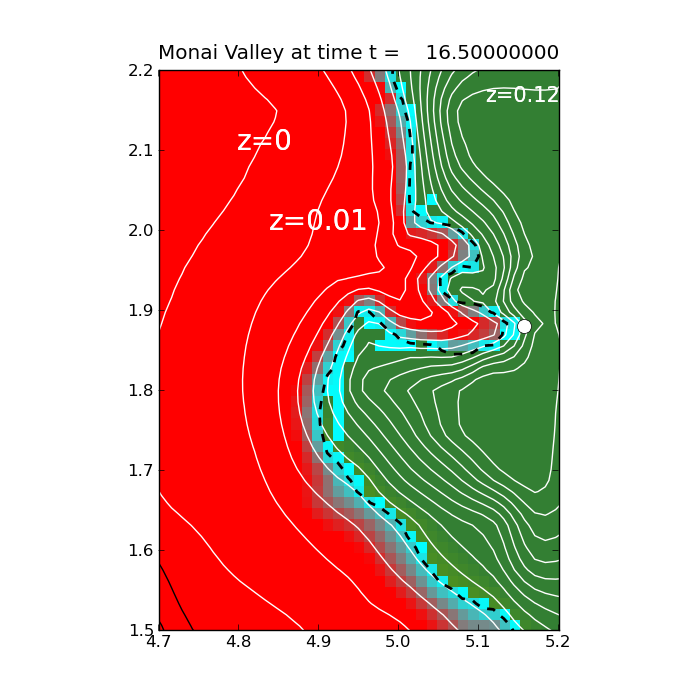
\includegraphics[width=5.4in]{bp7/figs423/contours.png}\hfil

\caption{\label{fig:bp7gauges}   %% choose appropriate label
% Use label fig:bp?text and then you can refer to as \Fig{bp?text} later.
Add a caption
  }
\end{figure}



%%% Add other subsections as needed.


\subsection{Lessons learned}

\todo{Make any relevant comments or observation regarding the benchmark itself,
the available data provided, the relevance of the benchmark to tsunami
science in general and to validating your specific model in particular. 
Report problems and make recommendations regarding improving the benchmark
or its data, as appropriate.}




